\chapter{TINJAUAN PUSTAKA}
\label{chap:tinjauanpustaka}

% Ubah bagian-bagian berikut dengan isi dari tinjauan pustaka

Demi mendukung penelitian ini, dibutuhkan beberapa teori penunjang sebagai bahan acuan dan refrensi. Dengan demikian penelitian ini menjadi lebih terarah.

\section{Dasar Teori}
\label{sec:dasarteori}

\subsection{\textit{Artificial Intelligence}}
\label{subsec:artificial-itelligence}

\textit{Artificial Intelligence} mengacu pada simulasi kecerdasan manusia dalam mesin yang diprogram untuk berpikir seperti manusia dan meniru tindakan mereka.\citep{artificialintellingece} Istilah ini juga dapat diterapkan pada mesin apa pun yang menunjukkan ciri-ciri yang terkait dengan pikiran manusia seperti pembelajaran dan pemecahan masalah.

Karakteristik ideal dari \textit{artificial intellingence} adalah kemampuannya untuk merasionalisasi dan mengambil tindakan yang memiliki peluang terbaik untuk mencapai tujuan tertentu. Bagian dari \textit{artificial intellingece} adalah \textit{machine learning}, yang mengacu pada konsep bahwa program komputer dapat secara otomatis belajar dari dan beradaptasi dengan data baru tanpa dibantu oleh manusia. Teknik\textit{deep learning} memungkinkan pembelajaran otomatis ini melalui penyerapan sejumlah besar data tidak terstruktur seperti teks, gambar, atau video.

\subsection{\textit{Machine Learning}}
\label{subsec:machine-learning}

\textit{Machine Learning} adalah studi tentang algoritma komputer yang memberikan sistem kemampuan untuk belajar secara otomatis dan dapat meningkatkan kemampuan dari pengalaman yang sudah didapatkan \citep{machinelearning1}. Hal ini umumnya dilihat sebagai sub-bidang kecerdasan buatan. Algoritma pembelajaran mesin memungkinkan sistem membuat keputusan secara mandiri tanpa dukungan eksternal. Keputusan semacam itu dibuat dengan menemukan pola dasar yang berharga dalam data yang kompleks. Berdasarkan pendekatan pembelajaran, jenis data \textit{input} dan \textit{output}, dan jenis masalah yang dipecahkan, ada beberapa kategori utama dari algoritma \textit{machine learning} \textit{supervised, unsupervised} dan \textit{reinforcement learning}. Ada beberapa pendekatan hibrida dan metode umum lainnya yang menawarkan ekstrapolasi alami dari bentuk masalah pembelajaran mesin. Berikut merupakan penjelasan dari beberapa kategori utama dari algoritma \textit{machine learning}:

\begin{enumerate}
	\item \textit{Supervised Learning} diterapkan ketika data dalam bentuk variabel input dan nilai target output. Algoritma akan mempelajari fungsi pemetaan dari \textit{input} ke \textit{output}. Ketersediaan sampel data berlabel dengan skala besar mempunyai nilai yang tinggi dikarenakan masih terdapat kelangkaan \textit{dataset}. Pendekatan ini secara luas dapat dibagi menjadi dua kategori utama yaitu \textit{classification} dan \textit{regression}. Gambar \ref{fig:supervised} menampilkan visualisasi dari \textit{classification} dan \textit{regression} pada \textit{Supervised Learning}
	
	\begin{figure}[ht]
		\centering
		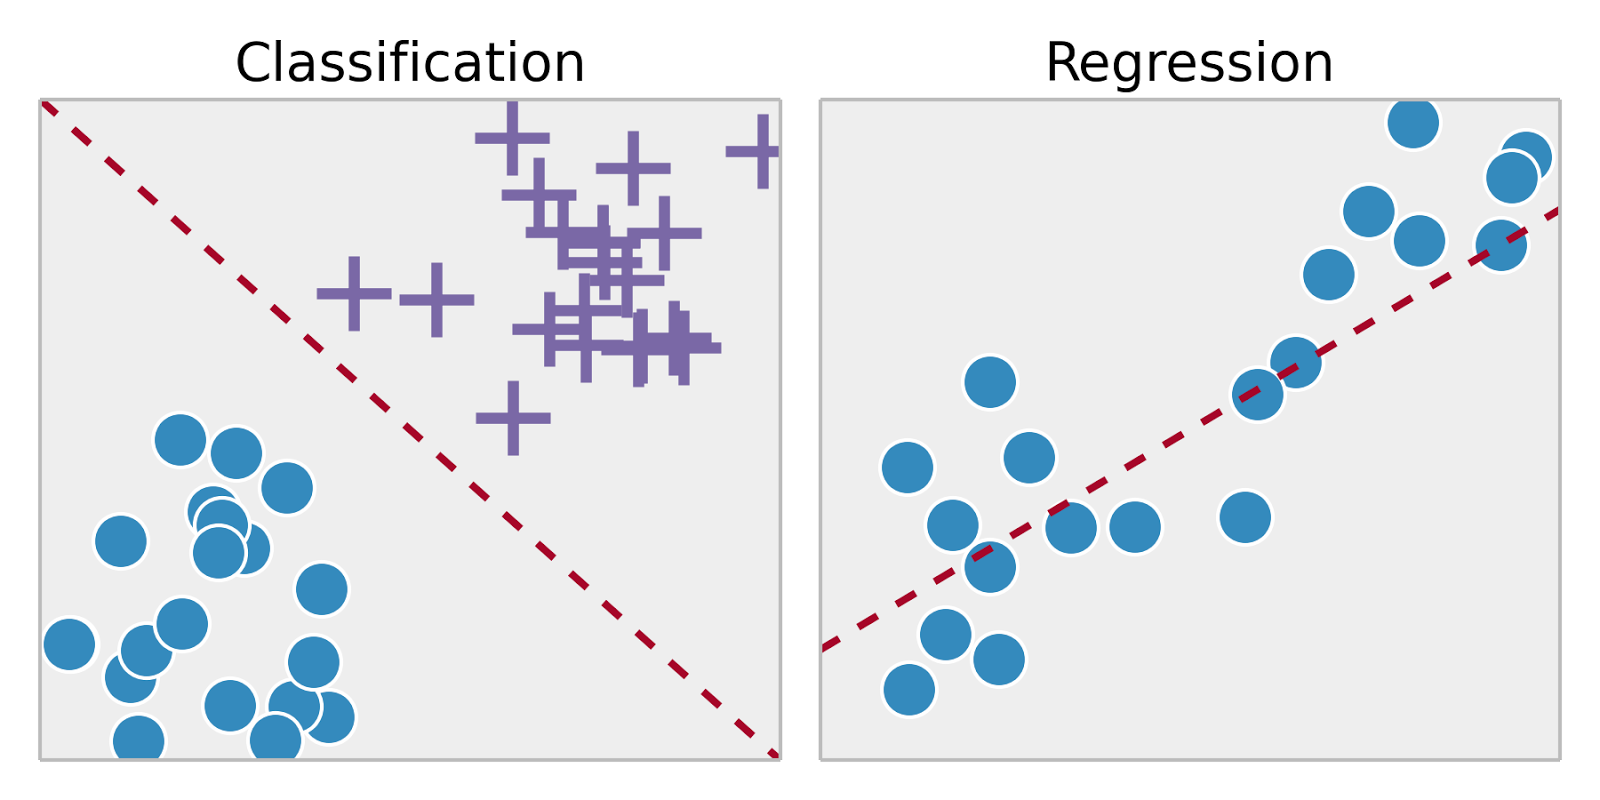
\includegraphics[scale=0.1]{gambar/supervised.png}
		\caption{Gambaran \textit{Supervised Learning}\citep{supervised}}
		\label{fig:supervised}
	\end{figure}  
	
	\item \textit{Unsupervised Learning} diterapkan ketika data hanya tersedia dalam bentuk \textit{input} dan tidak ada variabel \textit{output} yang sesuai. Algoritma semacam itu memodelkan pola yang mendasari data untuk mempelajari lebih lanjut tentang karakteristiknya. Salah satu jenis utama dari algoritma \textit{unsupervised} adalah pengelompokan. Dalam teknik ini, kelompok yang melekat dalam data ditemukan dan kemudian digunakan untuk memprediksi \textit{output} untuk \textit{input} yang tidak terlihat. Contoh dari teknik ini adalah untuk memprediksi perilaku pembelian pada pelanggan. Gambar \ref{fig:unsupervised} merupakan visualisasi dari algoritma \textit{unsupervised learning}.
	
	\begin{figure}[ht]
		\centering
		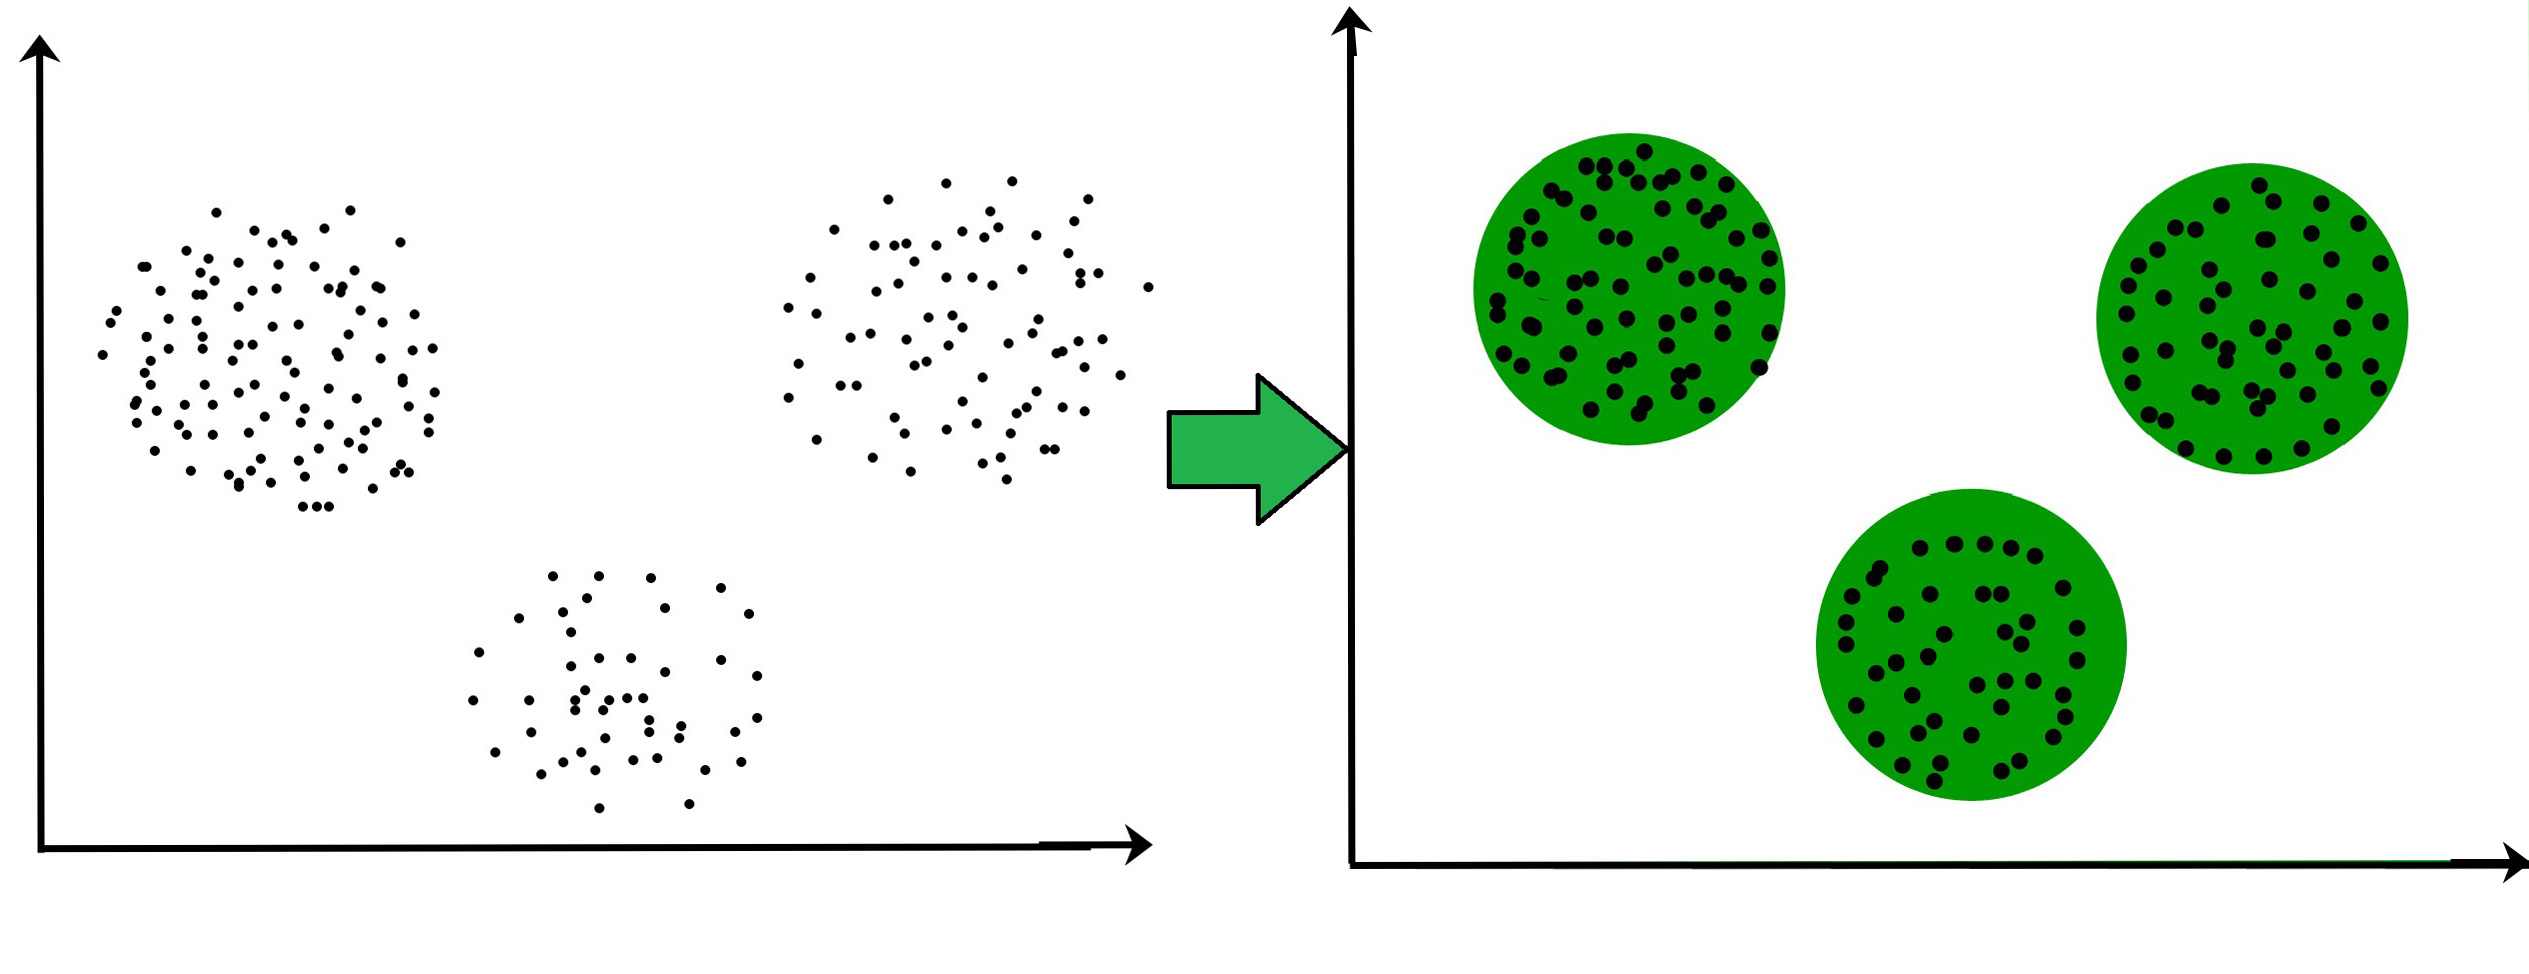
\includegraphics[scale=0.2]{gambar/unsupervised.jpg}
		\caption{Gambaran \textit{Unsupervised Learning}\citep{unsupervised}}
		\label{fig:unsupervised}
	\end{figure}
	
	
	\item \textit{Reinforcement learning} diterapkan ketika tugas yang ada
	adalah membuat urutan keputusan menuju \textit{reward} akhir. Selama proses \textit{learning}, \textit{artificial agent} mendapat \textit{reward} atau \textit{penalties} atas tindakan yang dilakukannya. Tujuannya adalah untuk memaksimalkan total \textit{reward} yang didapatkan. Gambar \ref{fig:reinforcement} merupakan visualisasi dari algoritma \textit{reinforcement learning}.
	
	\begin{figure}[ht]
		\centering
		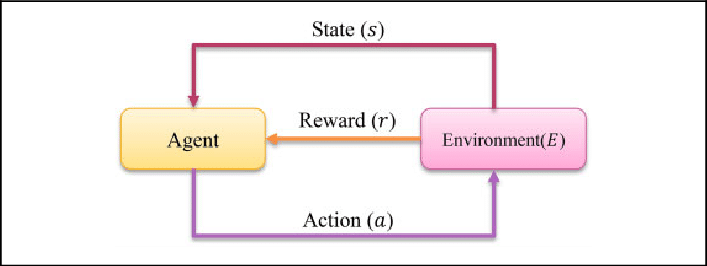
\includegraphics[scale=0.3]{gambar/reinforcement.png}
		\caption{Gambaran \textit{Reinforcement Learning}\citep{reinforcement}}
		\label{fig:reinforcement}
	\end{figure}
\end{enumerate}

\subsection{\textit{Deep Learning}}
\label{subsec:deeplearning}

\textit{Deep Learning} adalah kelas \textit{machine learning} yang berkinerja jauh lebih baik pada data tidak terstruktur\citep{dl}. Teknik \textit{deep learning} mengungguli teknik \textit{machine learning} saat ini. Ini memungkinkan model komputasi untuk mempelajari fitur secara progresif dari data di berbagai level. Popularitas \textit{deep learning} diperkuat karena jumlah data yang tersedia meningkat serta kemajuan perangkat keras yang menyediakan komputer yang kuat.

Arsitektur \textit{deep learning} berkinerja lebih baik daripada jaringan saraf tiruan  sederhana, meskipun waktu \textit{learning} dari struktur \textit{deep learning} lebih tinggi dari jaringan saraf tiruan. Namun, waktu \textit{learning} dapat dikurangi dengan menggunakan metode seperti \textit{transfer learning} atau komputasi menggunakan GPU. Salah satu faktor yang menentukan keberhasilan jaringan saraf terletak pada desain arsitektur jaringan yang cermat.

\subsection{\textit{Convolutional Neural Network}}
\label{subsec:cnn}

\textit{Convolutional Neural Networl} (CNN) adalah jenis khusus dari \textit{multilayer neural network} atau arsitektur \textit{deep learning} yang terinspirasi oleh sistem visual makhluk hidup \citep{cnn}. CNN sangat cocok untuk berbagai bidang visi komputer dan \textit{natural language processing}. \textit{Convolutional Neural Network} (CNN), juga disebut \textit{ConvNet}, adalah jenis \textit{Artificial Neural Network} (ANN), yang memiliki arsitektur \textit{feed-forward} yang dalam dan memiliki kemampuan generalisasi yang luar biasa dibandingkan dengan jaringan lain dengan lapisan FC (\textit{Fully Connected}), ia dapat mempelajari fitur objek yang sangat abstrak terutama data spasial dan dapat mengidentifikasinya dengan lebih efisien. Model CNN yang dalam terdiri dari satu set lapisan pemrosesan yang dapat mempelajari berbagai fitur data \textit{input} (misalnya gambar) dengan beberapa tingkat abstraksi seperti yang ditampilkan pada Gambar \ref{fig:concept-cnn}. Lapisan inisiator mempelajari dan mengekstrak fitur tingkat tinggi (dengan abstraksi yang lebih rendah), dan lapisan yang lebih dalam mempelajari dan mengekstrak fitur tingkat rendah (dengan abstraksi yang lebih tinggi).

\begin{figure}[ht]
	\centering
	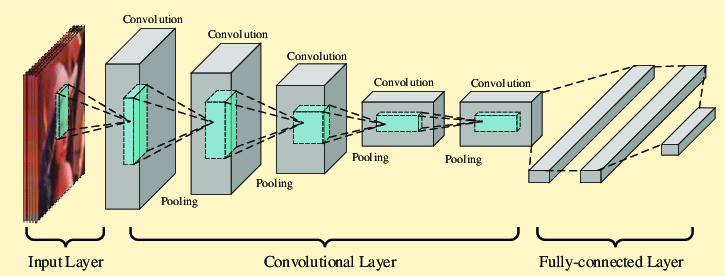
\includegraphics[scale=0.3]{gambar/concept-cnn.png}
	\caption{Gambaran Konsep Arsitektur CNN \citep{concept-cnn}}
	\label{fig:concept-cnn}
\end{figure}

\textit{Convolutional Neural Network} memiliki beberapa keunggulan dibanding dengan jaringan saraf tiruan lainnya dalam konteks visi komputer, antara lain :

\begin{enumerate}
	\item Salah satu alasan utama untuk mempertimbangkan CNN dalam kasus tersebut adalah fitur pembagian bobot dari CNN, yang mengurangi jumlah parameter yang dapat dilatih dalam jaringan, yang membantu model untuk menghindari \textit{overfitting} dan juga untuk meningkatkan generalisasi.
	\item Pada CNN, lapisan klasifikasi dan lapisan ekstraksi fitur melakukan proses \textit{learning} secara bersama-sama, yang membuat output model lebih terorganisir dan membuat output lebih bergantung pada fitur yang diekstraksi.
	\item Implementasi pada jaringan dengan ukuran yang besar akan lebih sulit dilakukan dengan menggunakan jenis jaringan saraf lain daripada menggunakan \textit{Convolutional Neural Network}
\end{enumerate}

\subsection{\textit{Convolutional Layer}}
\label{subsec:convolutional-layer}

\textit{Convolutional layer} adalah komponen terpenting dari arsitektur CNN mana pun. Ini berisi satu set kernel convolutional (juga disebut filter), yang dililitkan dengan gambar input (metrik N-dimensi) untuk menghasilkan peta fitur keluaran. Kernel dapat digambarkan sebagai kisi nilai atau angka diskrit, di mana setiap nilai dikenal sebagai bobot kernel. Selama awal proses pelatihan model CNN, semua bobot kernel ditetapkan dengan angka acak (pendekatan yang berbeda juga tersedia untuk inisialisasi bobot). Kemudian, dengan setiap periode \textit{learning}, bobot disetel dan kernel belajar mengekstrak fitur yang memberikan informasi mengenai data.

Pada \textit{Convolutional layer} terdapat istilah kernel yang mempunyai peran penting dalam proses yang dinamakan \textit{convolutional operation}. Kernel dapat digambarkan sebagai kisi nilai atau angka diskrit, di mana setiap nilai dikenal sebagai bobot kernel ini. Selama awal proses pelatihan model CNN, semua bobot kernel ditetapkan dengan angka acak (pendekatan yang berbeda juga tersedia di sana untuk menginisialisasi bobot). Kemudian, dengan setiap periode pelatihan, bobot disetel dan kernel belajar mengekstrak fitur yang berarti.

Sebelum kita mempelajari lebih jauh, mari kita pahami dulu format \textit{input} CNN. Berbeda dengan \textit{neural network} klasik lainnya dimana \textit{input}-nya dalam format vektor, di CNN \textit{input}-nya adalah gambar multi \textit{channel}. Misalnya untuk gambar RGB seperti pada Gambar \ref{fig:rgb-gray-image} mempunyai 3 \textit{channel} dan untuk gambar \textit{grayscale} hanya mempunyai satu \textit{channel}.

\begin{figure}[ht]
	\centering
	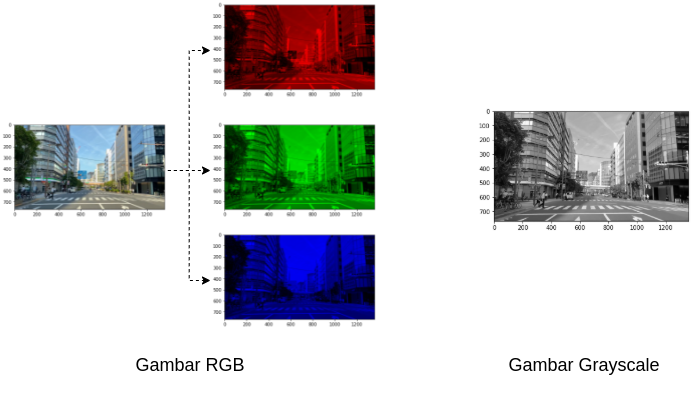
\includegraphics[scale=0.3]{gambar/rgb-gray-image.png}
	\caption{Contoh Gambar RGB dan Grayscale}
	\label{fig:rgb-gray-image}
\end{figure}

Sekarang, dalam operasi konvolusi, sebagai contoh diambil kernel 2 $\times$ 2 lalu diimplementasikan ke semua gambar 4 $\times$ 4 secara horizontal maupun vertikal dan sepanjang proses berlangsung dilakukan \textit{dot product} antara kernel dan gambar \textit{input} dengan mengalikan nilai yang sesuai dari keduanya dan dijumlahkan semua nilai untuk menghasilkan satu nilai skalar di \textit{feature map output}.Proses ini berlanjut hingga kernel tidak dapat lagi digeser lebih jauh. Untuk memahaminya secara lebih jelas, mari kita lakukan beberapa perhitungan awal yang dilakukan pada setiap langkah secara grafis seperti yang ditunjukkan pada Gambar \ref{fig:conv-step}, di mana setiap nilai kernel 2 $\times$ 2 (ditunjukkan dengan warna merah) berada dikalikan dengan wilayah berukuran sama (ditunjukkan dengan warna jingga) dalam gambar input 4 $\times$ 4 dan nilai yang dihasilkan dijumlahkan untuk mendapatkan entri yang sesuai (ditunjukkan dengan warna biru) di \textit{feature map output} pada setiap langkah konvolusi.

\begin{figure}[h!]
	\centering
	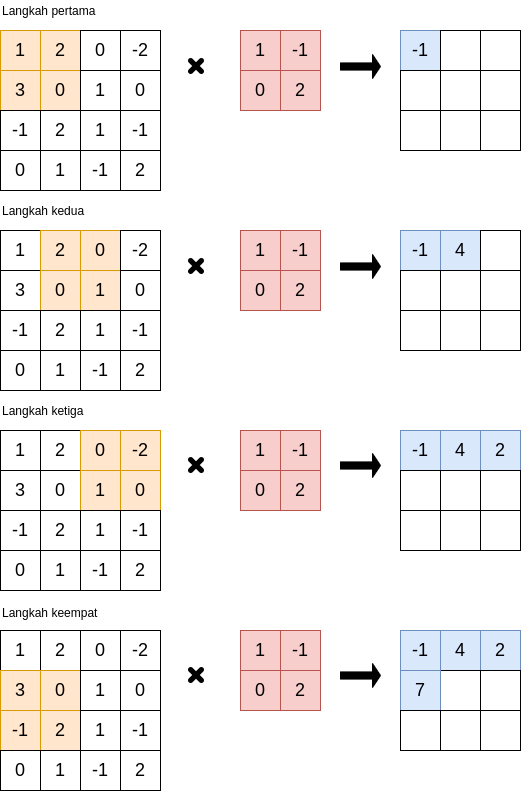
\includegraphics[scale=0.23]{gambar/langkah-konvolusi.png}
	\caption{Gambaran Operasi Konvolusi pada \textit{Convolution Layer}}
	\label{fig:conv-step}
\end{figure}

Dalam contoh di atas, diterapkan operasi konvolusi tanpa padding ke gambar masukan dan dengan \textit{stride} (yaitu ukuran langkah yang diambil sepanjang posisi horizontal atau vertikal ) sama dengan 1 ke kernel. Tapi bisa digunakan nilai \textit{stride} lain (bukan 1) dalam operasi konvolusi. Hal yang terlihat adalah jika kita meningkatkan langkah operasi konvolusi, itu menghasilkan \textit{feature map} berdimensi lebih rendah. \textit{Padding} penting untuk memberikan informasi ukuran batas dari input gambar jika tidak, tanpa menggunakan \textit{padding} apa pun, fitur sisi tepi akan terhapus terlalu cepat. \textit{Padding} juga digunakan untuk meningkatkan ukuran gambar \textit{input}, akibatnya ukuran \textit{feature map} \textit{output} juga meningkat. Gambar \ref{fig:conv-step-padd} memberikan contoh dengan menunjukkan operasi konvolusi dengan \textit{Zero-padding} dan 3 \textit{stride}. Rumus untuk mencari ukuran \textit{feature map} keluaran setelah operasi konvolusi adalah sebagai berikut:

\begin{equation}
	h'= \left[ \frac{h-f+p}{s} +1 \right]  
\end{equation}

\begin{equation}
	w'= \left[ \frac{w-f+p}{s} +1 \right]
\end{equation}

Dimana $h'$ menunjukkan tinggi dari \textit{feature map output}, $w'$ menunjukkan lebar dari \textit{feature map output}, $h$ menunjukkan tinggi dari gambar \textit{input}, $w$ menunjukkan lebar dari gambar \textit{input}, $f$ adalah ukuran filter, $p$ menunjukkan \textit{padding} dari operasi konvolusi dan $s$ menunjukkan \textit{stride} operasi konvolusi.

\begin{figure}[h!]
	\centering
	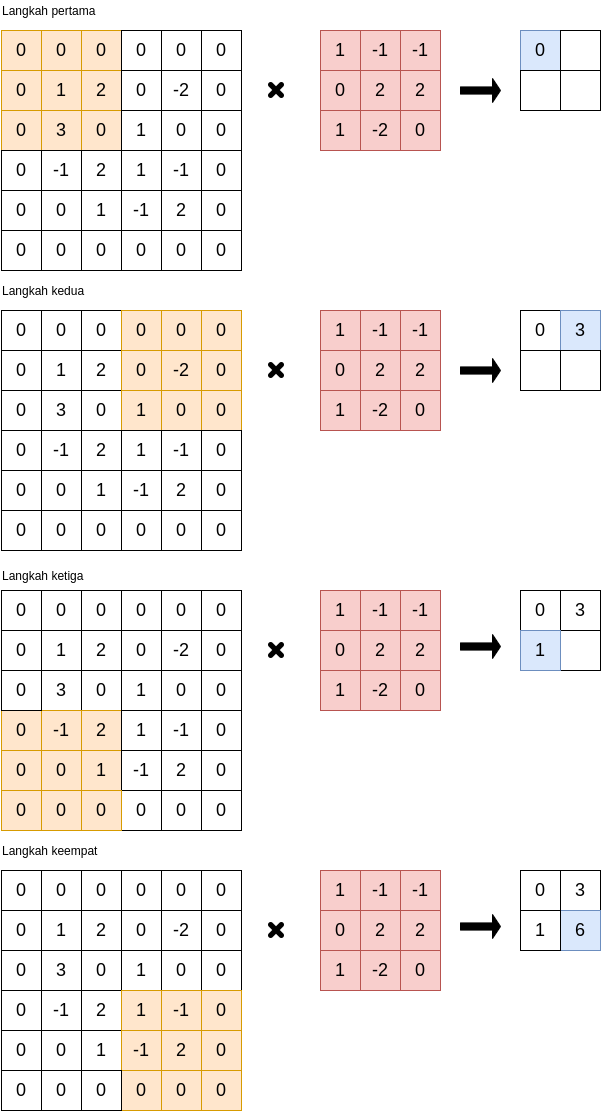
\includegraphics[scale=0.25]{gambar/conv-step-padd.png}
	\caption{Gambaran Operasi Konvolusi pada \textit{Convolution Layer} menggunakan \textit{Zero Padding}}
	\label{fig:conv-step-padd}
\end{figure}

Keuntungan utama dari lapisan konvolusi adalah:
\begin{enumerate}
	\item \textbf{\textit{Sparse Connectivity}}: Dalam jaringan saraf yang terhubung penuh, setiap \textit{neuron} dari satu lapisan terhubung dengan setiap \textit{neuron} dari lapisan berikutnya tetapi di CNN sejumlah kecil bobot terdapat di antara dua lapisan. Akibatnya, jumlah koneksi atau bobot yang kita butuhkan kecil, dan jumlah memori untuk menyimpan bobot itu juga kecil, sehingga hemat dalam penggunaan memori. Selain itu, operasi dot(.) secara komputasi lebih ringan daripada perkalian matriks.
	\item \textbf{\textit{Weight Sharing}}: Di CNN, tidak ada bobot khusus yang ada di antara dua neuron dari lapisan yang berdekatan melainkan semua bobot bekerja dengan setiap piksel dari matriks \textit{input}.Selain mempelajari bobot baru untuk setiap neuron, kita dapat mempelajari satu set bobot untuk semua input dan hal ini secara drastis dapat mengurangi waktu pelatihan.
\end{enumerate}

\subsection{\textit{Pooling Layer}}
\label{subsec:pooling-layer}

\textit{Pooling layer} digunakan untuk membuat sub-sampel \textit{feature map} (dihasilkan setelah operasi konvolusi), yaitu mengambil \textit{feature map} berukuran lebih besar dan mengecilkannya menjadi \textit{feature map} berukuran lebih kecil. Saat menyusutkan \textit{feature map}, \textit{pooling layer} tetap mempertahankan fitur (atau informasi) yang paling dominan di setiap langkah \textit{pools}. Operasi \textit{pooling} dilakukan dengan menentukan ukuran \textit{pooled region} dan langkah operasi, mirip dengan operasi konvolusi. Ada berbagai jenis teknik \textit{pooling} yang digunakan dalam berbagai \textit{pooling layer} seperti \textit{max pooling, min pooling, average pooling, gated pooling, tree pooling}, dan lain-lain. \textit{Max Pooling} adalah teknik pooling yang paling populer dan banyak digunakan.

Kelemahan utama dari \textit{pooling layer} adalah terkadang menurunkan kinerja CNN secara keseluruhan. Alasan di balik ini adalah bahwa lapisan penyatuan membantu CNN untuk menemukan apakah fitur tertentu ada dalam gambar masukan yang diberikan atau tidak tanpa memperhatikan posisi yang tepat dari fitur tersebut.

Gambar \ref{fig:max-pooling} mengilustrasikan contoh yang menunjukkan beberapa langkah awal serta keluaran akhir dari operasi \textit{max-pooling}, di mana ukuran area \textit{pooling} adalah 2 $\times$ 2 (ditunjukkan dalam warna jingga, dalam \textit{feature map input}) dengan \textit{stride} sama dengan 1 dan yang sesuai dihitung nilai di \textit{feature map output}. Rumus untuk menemukan ukuran \textit{feature map output} setelah operasi \textit{pooling} seperti di bawah ini:

\begin{figure}[h!]
	\centering
	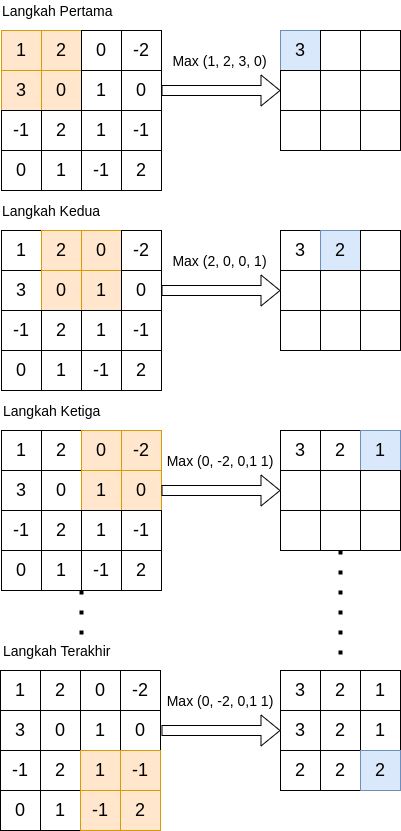
\includegraphics[scale=0.25]{gambar/max-pooling.png}
	\caption{Gambaran Proses \textit{Max Pooling}}
	\label{fig:max-pooling}
\end{figure}

\begin{equation}
	h'= \left[ \frac{h-f}{s} \right]
\end{equation}

\begin{equation}
	w'= \left[ \frac{w-f}{s} \right]
\end{equation}

Dimana $h'$ menunjukkan tinggi dari \textit{feature map output}, $w'$ menunjukkan lebar dari \textit{feature map output}, $h$ menunjukkan tinggi dari gambar \textit{input}, $w$ menunjukkan lebar dari gambar \textit{input}, $f$ adalah ukuran area \textit{pooling}, $s$ menunjukkan \textit{stride} operasi \textit{pooling}.

\subsection{Fungsi Aktivasi (\textit{Non-Linearity})}
\label{subsec:fungsi-aktivasi}

Tugas utama dari setiap fungsi aktivasi dalam setiap model berbasis jaringan saraf adalah untuk memetakan \textit{input output}, di mana nilai \textit{input} diperoleh dengan menghitung jumlah terbobot \textit{input neuron} dan selanjutnya menambahkan bias (jika ada bias). Dengan kata lain, fungsi aktivasi memutuskan apakah neuron akan aktif atau tidak untuk \textit{input} yang diberikan dengan menghasilkan \textit{output} yang sesuai. Terdapat beberapa fungsi aktivasi yang digunakan dalam CNN, antara lain :

\begin{enumerate}
	\item \textbf{Sigmoid}\\
	Fungsi aktivasi sigmoid mengambil bilangan real sebagai inputnya dan mengikat outputnya dalam kisaran [0,1]. Kurva fungsi sigmoid berbentuk 'S' seperti pada Gambar \ref{fig:sigmoid}. Representasi tematik dari sigmoid adalah:
	
	\begin{equation}
		f(x)_{sigm}=\frac{1}{1+e^{-x}}
	\end{equation}
	
	\begin{figure}[h!]
		\centering
		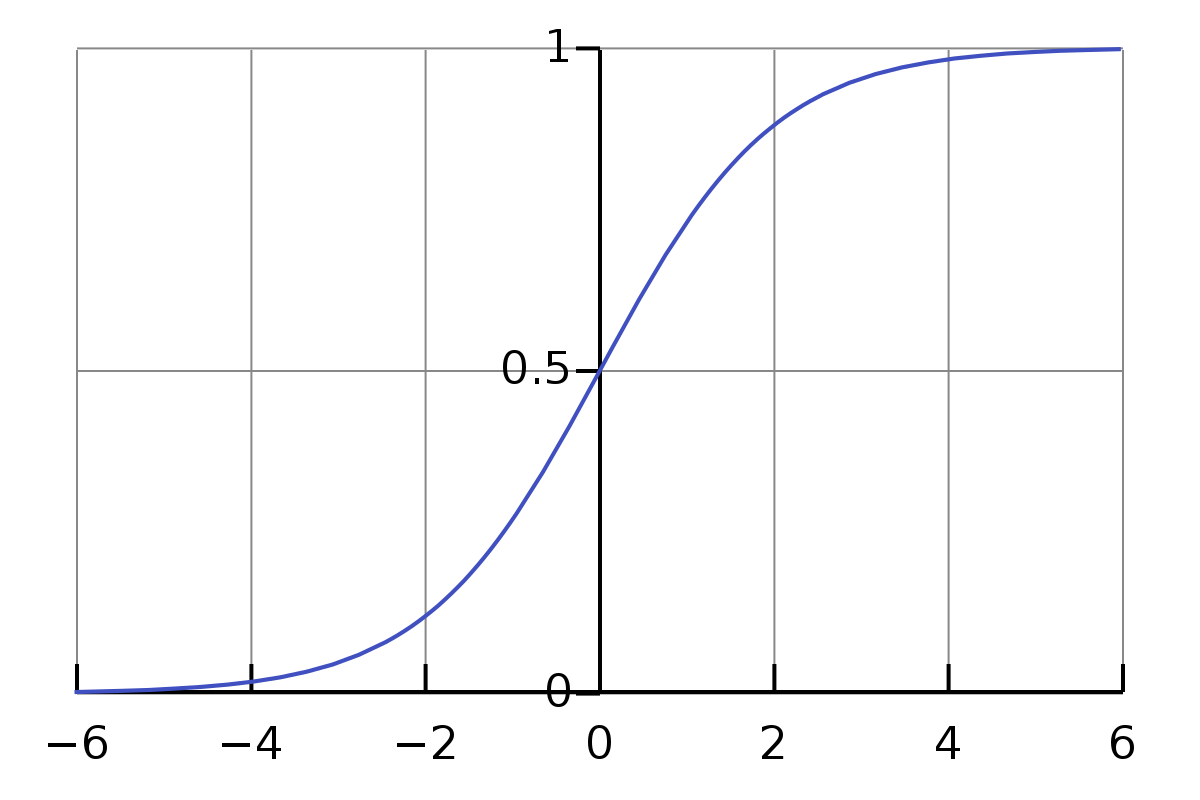
\includegraphics[scale=0.15]{gambar/sigmoid.png}
		\caption{Grafik Fungsi Aktivasi Sigmoid \citep{sigmoid}}
		\label{fig:sigmoid}
	\end{figure}
	
	\item \textbf{Tanh}\\
	Fungsi aktivasi Tanh digunakan untuk mengikat nilai input (bilangan real) dalam kisaran [-1,1] seperti tertampil pada Gambar \ref{fig:tanh}. Representasi matematis dari Tanh adalah:
	
	\begin{equation}
		f(x)_{tanh}=\frac{e^x-e^{-x}}{e^x+e^{-x}}
	\end{equation}
	
	
	\begin{figure}[h!]
		\centering
		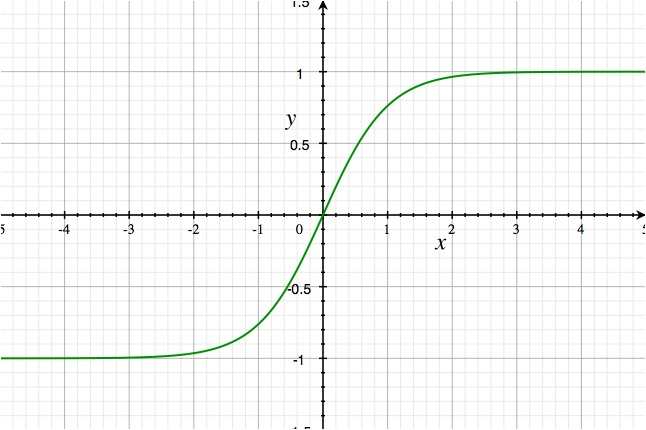
\includegraphics[scale=0.25]{gambar/tanh.jpg}
		\caption{Grafik Fungsi Aktivasi Tanh \citep{sigmoid}}
		\label{fig:tanh}
	\end{figure}
	
	\item \textbf{ReLU} \\
	Rectifier Linear Unit (ReLU) adalah fungsi aktivasi yang paling umum digunakan dalam Convolutional Neural Networks. Ini digunakan untuk mengubah semua nilai input menjadi bilangan positif. Keuntungan dari ReLU adalah membutuhkan beban komputasi yang sangat minimal dibandingkan dengan yang lain. Representasi matematis dari ReLU adalah:
	\begin{equation}
		f(x)_{ReLU}=\textbf{max}(0,x)
	\end{equation}
	
	Namun terkadang ada beberapa masalah besar dalam menggunakan fungsi aktivasi ReLU. Misalnya, jika terdapat gradient yang besar pada saat pencarian \textit{error} dengan menggunakan algortima \textit{back propagation}. Gradien yang besar ini apabila dilewatkan melalui fungsi ReLU, dapat menyebabkan bobot akan diperbarui sedemikian rupa sehingga neuron tidak pernah diaktifkan lagi. Masalah ini dikenal sebagai masalah \textit{"Dying ReLU"}. Untuk mengatasi masalah ini ada beberapa varian ReLU yang tersedia, diantaranya adalah Leaky ReLU dan Noisy ReLU. Tidak seperti ReLU, fungsi aktivasi Leaky ReLU tidak mengabaikan input negatif sepenuhnya, melainkan menurunkan skala input negatif tersebut. Leaky ReLU digunakan untuk menyelesaikan masalah \textit{Dying ReLU}. Representasi matematis dari Leaky ReLU adalah
	
	\begin{equation}
		f(x)_{LeakyReLU} =
		\begin{cases}
			x, & \text{if x$>$0}\\
			mx, & \text{if x$\leq$0}\\
		\end{cases}       
	\end{equation}  
	Di mana $m$ adalah konstanta, yang disebut faktor kebocoran dan umumnya disetel ke nilai kecil (seperti 0,001). Sedangkan Noisy ReLU digunakan distribusi Gaussian untuk membuat ReLU \textit{noisy}. Representasi matematis dari Noise ReLU adalah
	
	\begin{equation}
		f(x)_{NoisyReLU} = \textbf{max}(x + Y) , \textit{with} Y \sim N(0,\sigma(x))
	\end{equation}
	
\end{enumerate}

\subsection{Fully Connected Layer}
\label{subsec:fcn}

Biasanya bagian terakhir (atau lapisan) dari setiap arsitektur CNN (digunakan untuk klasifikasi) terdiri dari \textit{fully-connected layers}, di mana setiap neuron di dalam lapisan terhubung dengan setiap neuron dari lapisan sebelumnya. Lapisan terakhir dari lapisan \textit{Fully-Connected} digunakan sebagai lapisan keluaran (\textit{classifier}) dari arsitektur CNN. Lapisan \textit{Fully-Connected} adalah jenis jaringan saraf tiruan \textit{feed-forward} (ANN) dan mengikuti prinsip tradisional \textit{Multi-Layer Perceptron neural network} (MLP). Layer FC mengambil \textit{input} dari c\textit{onvolutional} atau \textit{pooling layer} akhir, yang berupa sekumpulan metrik (\textit{feature map}) dan matrik tersebut diratakan (\textit{flatten}) untuk membuat vektor dan vektor ini kemudian dimasukan ke dalam layer FC untuk menghasilkan hasil akhir \textit{output} CNN.

\subsection{\textit{Loss Function}}
\label{subsec:lossfunction}

Pada \textit{output layer}, dilakukan perhitungan kesalahan prediksi yang dihasilkan oleh model CNN atas sampel \textit{learning} menggunakan beberapa \textit{Loss Function}. \textit{Error} prediksi ini memberitahu jaringan bagaimana prediksinya dari \textit{output} aktual, dan kemudian \textit{error} ini akan dioptimalkan selama proses \textit{learning} model CNN. \textit{Loss function} menggunakan dua parameter untuk menghitung \textit{error}, parameter pertama adalah \textit{output} estimasi dari model CNN (juga disebut prediksi) dan yang kedua adalah \textit{output} aktual (juga dikenal sebagai label). Berikut adalah beberapa contoh \textit{loss function} yang banyak digunakan dalam algoritma \textit{deep learning}:


\begin{enumerate}
	\item \textit{\textbf{Cross-Entropy Loss Function}}\\
	\textit{Cross-entropy loss}, juga disebut fungsi \textit{log loss} banyak digunakan untuk mengukur kinerja model CNN, yang outputnya adalah probabilitas $p \in \{0,1\}$. \textit{Loss Function} ini banyak digunakan sebagai alternatif dari \textit{squared error loss function} dalam masalah klasifikasi multi-kelas. \textit{Cross-entropy loss} menggunakan aktivasi softmax di lapisan \textit{output} untuk menghasilkan \textit{output} dalam distribusi probabilitas, yaitu $p, y \in R^N$, di mana $p$ adalah probabilitas untuk setiap kategori \textit{output} dan $y$ menunjukkan \textit{output} yang diinginkan dan probabilitas setiap kelas \textit{output} dapat diperoleh dengan : 
	
	\begin{equation}
		p_i = \frac{e^{a_i}}{\sum_{k=1}^{N} e^{a_k}}
	\end{equation}
	
	Di mana $N$ adalah jumlah neuron di lapisan \textit{output} dan $e^{a_i}$ menunjukkan setiap \textit{output} yang tidak dinormalisasi dari lapisan sebelumnya dalam jaringan. Lalu, \textit{cross-entropy loss} dapat didefinisikan sebagai:
	
	\begin{equation}
		H(p,y) =-\sum_{i} y_i\log(p_i)
	\end{equation}
	\begin{center}
		dimana $i \in \left[1,N\right]$
	\end{center}
	
	\item \textbf{\textit{Euclidean Loss Function}}\\
	\textit{Euclidean Loss} juga disebut \textit{mean squared loss }banyak digunakan dalam masalah regresi. \textit{Mean squared loss} antara \textit{output} yang diprediksi $p \in R^N$ dan output aktual $y \in R^N$ di setiap neuron dari lapisan \textit{output} CNN didefinisikan sebagai :
	
	\begin{equation}
		H(p,y)=\frac{1}{2N} \sum_{i=1}^{N} (p_i-y_i)^2
	\end{equation}
	
	\item \textit{\textbf{Hinge Loss Function}}\\
	\textit{Hinge Loss} banyak digunakan dalam masalah klasifikasi biner. Ini digunakan dalam masalah klasifikasi berbasis "margin maksimum", terutama untuk \textit{support vector machine} (SVM). Di sini, \textit{optimizer} mencoba memaksimalkan margin antara dua kelas target. Hinge Loss Function didefinisikan sebagai:
	
	\begin{equation}
		H(p,y) = \sum_{i=1}^{N} \textbf{max}(0, m-(2y_i - 1)p_i)
	\end{equation}

	Dimana $m$ adalah margin yang biasanya bernilai sama dengan 1, dan $p_i$ menunjukkan prediksi \textit{output} dan $y_i$ menunjukkan output yang diinginkan
		
\end{enumerate}

\subsection{\textit{Regional-Based CNN}}
\label{subsec:rcnn}

Semenjak\textit{ Convolution Neural Network} (CNN) dengan \textit{fully connected layer} tidak mampu menangani frekuensi kemunculan dan multi objek. Salah satu cara untuk mengatasinya adalah dengan menggunakan \textit{sliding window brute force search} untuk memilih wilayah dan menerapkan model CNN pada area tersebut, tetapi masalah dari pendekatan ini adalah bahwa objek yang sama dapat direpresentasikan dalam gambar dengan ukuran dan aspek rasio yang berbeda. Dengan mempertimbangkan faktor-faktor tersebut, penerapan algoritma \textit{deep learning} (CNN) pada jumlah \textit{region proposal} yang banyak akan menyebabkan proses komputasi yang dijalankan akan menjadi sangat berat dan rumit.

\begin{figure}[h!]
	\centering
	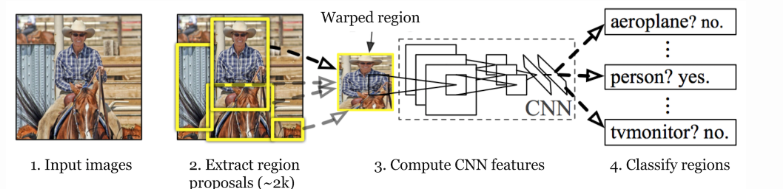
\includegraphics[scale=0.3]{gambar/rcnn.png}
	\caption{Arsitektur R-CNN \citep{arch-rcnn}}
	\label{fig:rcnn}
\end{figure}

Ross Girshick dan kawan-kawan pada tahun 2013 mengusulkan arsitektur baru yang disebut R-CNN seperti pada Gambar \ref{fig:rcnn} (\textit{Regional-based CNN}) untuk menghadapi tantangan deteksi objek ini \citep{rcnn}. Arsitektur R-CNN menggunakan algoritma \textit{selective search} yang menghasilkan sekitar 2000 \textit{region proposal}. \textit{Regional proposal} ini kemudian diterapkan ke arsitektur CNN untuk menghitung jumlah fitur CNN. Fitur-fitur ini kemudian diteruskan dalam model SVM untuk mengklasifikasikan objek yang ada di \textit{region proposal}. Langkah selanjutnya adalah melakukan regresi pada \textit{bounding box} untuk mengetahui lokasi objek yang ada dalam gambar dengan lebih tepat. 

\subsection{\textit{Fast R-CNN}}
\label{subsec:fast-rcnn}

Fast R-CNN ditemukan atas metode yang telah ditemukan terlebih dahulu yaitu \textit{R-CNN} untuk mengklasifikasikan proposal objek secara efisien menggunakan \textit{deep convolutional network} \citep{fast-rcnn}. Dibandingkan dengan \textit{R-CNN}, \textit{Fast R-CNN} menggunakan beberapa inovasi untuk meningkatkan kecepatan \textit{learning} dan pengujian sekaligus meningkatkan akurasi deteksi. Fast R-CNN dapat menyelesaikan proses \textit{training} dengan jaringan VGG16 yang sangat dalam memeberikan hasil yang 9 kali lebih cepat dari R-CNN, 213 kali lebih cepat pada waktu pengujian, dan mencapai mAP yang lebih tinggi pada PASCAL VOC 2012. Dibandingkan dengan SPPnet, Fast R-CNN dapat menyelesaikan proses \textit{training} dengan VGG16 3x lebih cepat, pengujian 10x lebih cepat, dan lebih akurat.

Jika pada R-CNN \textit{region proposal} akan melalui proses konvolusi di CNN, sebaliknya pada \textit{Fast R-CNN} gambar \textit{input}-lah yang akan melalui proses konvolusi di CNN seperti yang ditampilkan pada Gambar \ref{fig:fast-rcnn}. Hasil dari konvolusi pada \textit{Fast R-CNN} berupa \textit{convolutional feature map} yang akan digunakan untuk identifikasi \textit{region proposal} dan menyatukannya ke dalam bentuk persegi. Selanjutnya dengan menggunakan layer \textit{ROI Pooling} akan dibentuk kembali menjadi ukuran yang tetap sehingga dapat dimasukan ke dalam \textit{fully conneceted network}. Pada proses deteksi kelas dari \textit{region proposal} dan juga nilai offset dari \textit{bounding box} digunakan \textit{softmax layer} dari \textit{ROI feature vector} yang telah dihasilkan pada proses sebelumnya.

\begin{figure}[h]
	\centering
	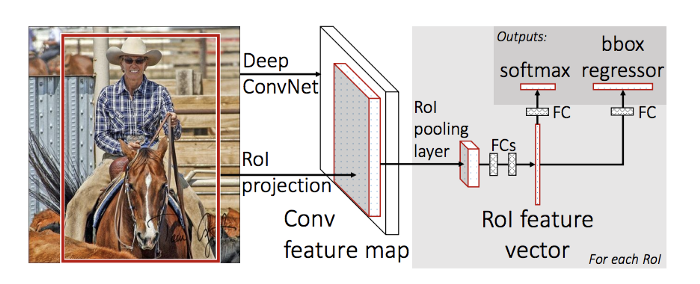
\includegraphics[scale=0.3]{gambar/fast-rcnn.png}
	\caption{Arsitektur \textit{Fast R-CNN} \citep{arch-fast-rcnn}}
	\label{fig:fast-rcnn}
\end{figure}

Alasan \textit{Fast R-CNN} lebih cepat daripada R-CNN adalah karena kita tidak perlu memasukkan 2000 \textit{region proposal} ke \textit{convolutional neural network} setiap saat. Sebagai gantinya, operasi konvolusi dilakukan hanya sekali per gambar dan \textit{feature map} dihasilkan operasi tersebut.

\subsection{\textit{Faster R-CNN}}
\label{subsec:faster-rcnn}

Pad kedua algoritma \textit{R-CNN} dan \textit{Fast R-CNN} menggunakan \textit{selective search} untuk mengetahui \textit{region proposal}. \textit{Selective search} sendiri memerlukan waktu yang cukup lama dalam penyelesain prosesnya sehingga mempengaruhi kinerja dari jaringan \citep{faster-rcnn}. Oleh karena itu, dibuatlah algoritma deteksi objek baru dengan menghilangkan algoritma \textit{selective search} dan memungkinkan jaringan mempelajari \textit{region proposal}.

Mirip dengan \textit{Fast R-CNN}, gambar dijadikann sebagai input ke jaringan konvolusi yang menyediakan \textit{convolusional feature map}. Disebabkan waktu eksekusi yang lama saat menggunakan algoritma \textit{selective search} pada \textit{feature map} untuk mengidentifikasi \textit{region proposal}, \textit{Faster R-CNN} menggunakan jaringan terpisah untuk memprediksi \textit{region proposal}. Jaringan terpisah ini dinamakan dengan \textit{Region Proposal Network (RPN)}, dimana \textit{RPN} berbagi \textit{full-image convolutional features} dengan jaringan deteksi yaitu \textit{Fast R-CNN}. \textit{Region proposal} yang diprediksi kemudian dibentuk kembali menggunakan \textit{ROI pooling layer} yang kemudian digunakan untuk mengklasifikasikan gambar di dalam \textit{region proposal} dan memprediksi nilai offset untuk \textit{bounding box}. Gambar \ref{fig:arch-faster-rcnn} merupakan visualisasi dari proses deteksi objek menggunakan \textit{Faster R-CNN}. 

\begin{figure}[h]
	\centering
	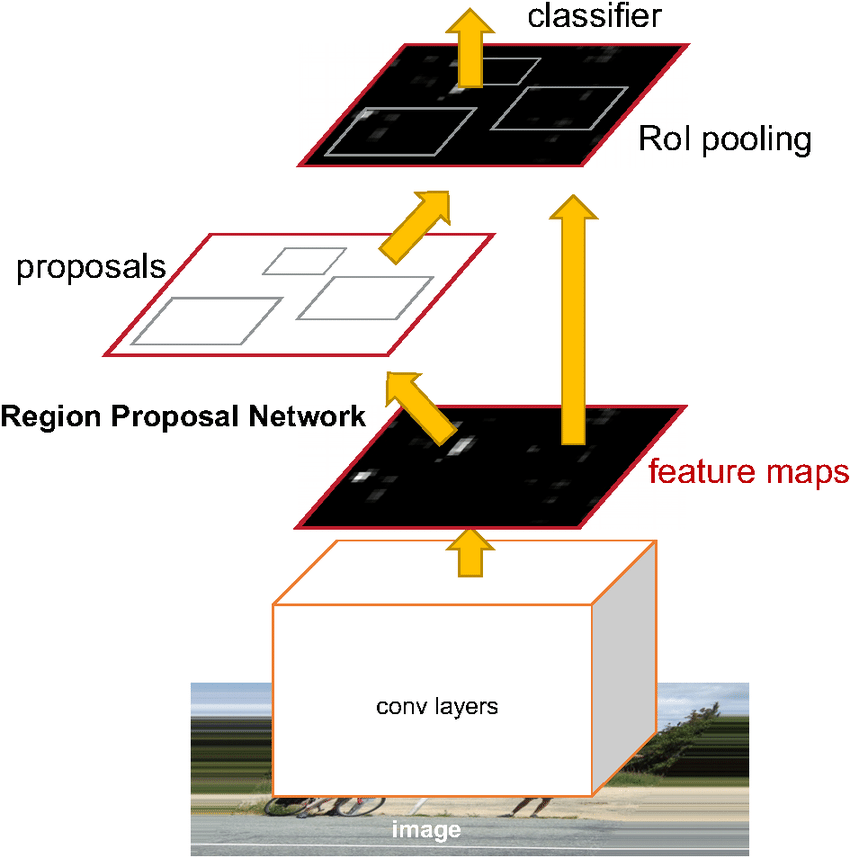
\includegraphics[scale=0.15]{gambar/arch-faster-rcnn.png}
	\caption{Gambaran Deteksi Objek pada \textit{Faster R-CNN} \citep{arch-faster-rcnn}}
	\label{fig:faster-rcnn}
\end{figure}

\subsection{\textit{Mask R-CNN}}
\label{subsec:mask-rcnn}

Mask R-CNN adalah Convolutional Neural Network (CNN) dan segmentasi citra termutakhir untuk saat ini. Varian Deep Neural Network ini mendeteksi objek dalam gambar dan menghasilkan \textit{mask} segmentasi berkualitas tinggi untuk setiap \textit{instance} \citep{mask-rcnn}. \textit{Mask R-CNN} dibangun menggunakan\textit{ Faster R-CNN} dimana \textit{Faster R-CNN} memiliki 2 \textit{output} untuk setiap objek, label kelas dan \textit{bounding box offset}. \textit{Mask R-CNN} adalah penambahan cabang ketiga yang mengeluarkan \textit{mask} objek seperti yang tertampil pada Gambar \ref{fig:arch-mask-rcnn}. \textit{output} \textit{mask} tambahan berbeda dari \textit{output} kelas dan \textit{bounding box}, yang membutuhkan ekstraksi tata letak spasial yang jauh lebih baik dari suatu objek.

\textit{Mask R-CNN} merupakan perpanjangan dari \textit{Faster R-CNN} dengan menambahkan cabang untuk memprediksi t\textit{mask} objek (\textit{Region of Interest}) secara paralel dengan cabang yang ada untuk pengenalan \textit{bounding box}. Satu keuntungan sederhana dari \textit{Mask R-CNN} dibandingkan \textit{Faster R-CNN} adalah kenyataan bahwa mudah untuk menggeneralisasi tugas lain seperti estimasi pose. Elemen kunci \textit{Mask R-CNN} adalah penyelarasan piksel-ke-piksel, yang merupakan bagian utama dari \textit{Fast/Faster R-CNN} yang hilang. \textit{Mask R-CNN} mengadopsi prosedur dua tahap yang sama dengan tahap pertama yang identik (yaitu \textit{RPN}). Pada tahap kedua, secara paralel untuk memprediksi kelas dan \textit{box offset}, Mask R-CNN juga mengeluarkan \textit{mask} biner untuk setiap \textit{RoI}. Ini berbeda dengan sistem terbaru, di mana klasifikasi bergantung pada prediksi \textit{mask}.

Mask R-CNN mudah diterapkan dan dilatih karena \textit{Faster R-CNN framework}, yang memfasilitasi berbagai desain arsitektur yang fleksibel. Selain itu, cabang \textit{mask} hanya menambahkan \textit{overhead} komputasi kecil, memungkinkan sistem dan eksperimen yang cepat.

\begin{figure}[h]
	\centering
	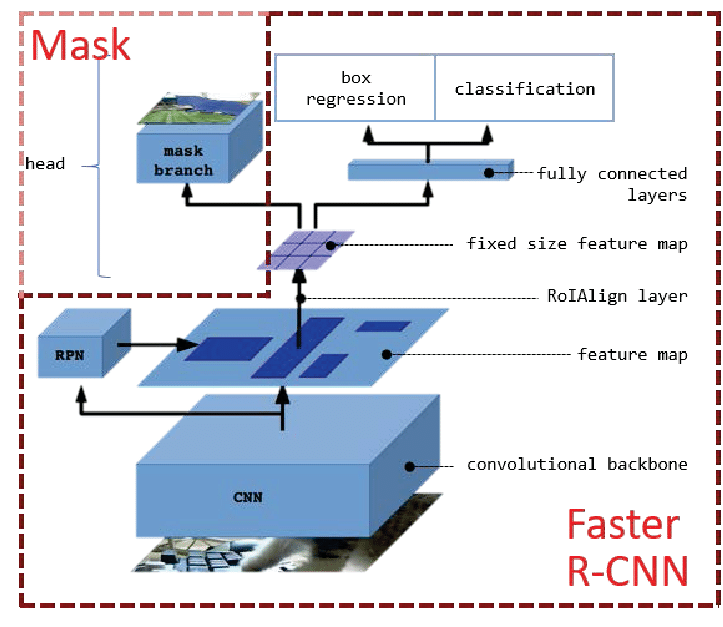
\includegraphics[scale=0.25]{gambar/arch-mask-rcnn.png}
	\caption{Struktur dari Arsitektur \textit{Faster R-CNN} \citep{arch-mask-rcnn}}
	\label{fig:mask-rcnn}
\end{figure}

\section{Penelitian Terkait}
\label{penelitianterkait}

\subsection{Real-Time Pedestrian Detection With Deep Network Cascades}
\label{realtime-pedestrian}

Penelitian ini dilakukan oleh Anelia Angelova dan kawan-kawan pada tahun 2015 yang menyajikan pendekatan real-time baru untuk deteksi objek yang mengeksploitasi efisiensi \textit{cascade classifiers} dengan akurasi \textit{deep neural network} \citep{penelitianterkait1}. \textit{Deep network} telah terbukti unggul dalam tugas klasifikasi, dan kemampuannya untuk beroperasi pada \textit{raw pixel input} tanpa perlu merancang fitur khusus. Namun, \textit{deep network} terkenal lambat pada waktu inferensi. Dalam \textit{paper} tersebut, Anelia Angelova dan kawan-kawan mengusulkan pendekatan \textit{cascades deep network} dan \textit{fast features}, yang sangat cepat dan sangat akurat. Mereka menerapkannya pada permasalahan pada deteksi pejalan kaki. Algoritma mereka berjalan secara real-time pada 15 frame per detik. Pendekatan yang dihasilkan mencapai tingkat kesalahan rata-rata 26,2\% pada \textit{benchmark} deteksi Caltech Pedestrian.

\subsection{Pedestrian Detection: The Elephant In The Room}
\label{pedestrian-detection}

Deteksi pejalan kaki digunakan di banyak aplikasi berbasis citra mulai dari pengawasan video hingga pengemudi otonom. Meskipun mencapai kinerja tinggi, sebagian besar masih belum diketahui seberapa baik detektor yang ada menggeneralisasi data yang tidak terlihat. Hal ini penting karena detektor yang praktis harus siap digunakan dalam berbagai skenario dalam aplikasi. Untuk tujuan tersebut, Irtiza Hasan dan kawan-kawan melakukan studi komprehensif dalam \textit{paper} ini, menggunakan prinsip umum evaluasi \textit{cross-dataset} langsung \citep{pedestrian-detection}. Melalui \textit{paper} ini, ditemukan bahwa detektor pejalan kaki terkini yang ada, meskipun berkinerja cukup baik ketika dilatih dan diuji pada kumpulan data yang sama, namun secara umum memiliki peforma yang cukup buruk dalam evaluasi \textit{cross-dataset}. 

Dalam \textit{paper} ini ditunjukkan bahwa ada dua alasan untuk permasalahan ini. Pertama, desain yang dibuat (misalnya, \textit{anchor settings}) mungkin bias terhadap tolok ukur dalam \textit{training} dan \textit{test pipeline} data tunggal, tetapi akibatnya sebagian besar membatasi kemampuan generalisasi dari keduanya. Kedua, sumber pelatihan umumnya tidak terlalu padat pada pejalan kaki dan mempunyi beragam dalam skenario. Di dalam evaluasi \textit{cross-dataset} langsung, secara mengejutkan, ditemukan bahwa detektor objek dengan tujuan umum, tanpa adaptasi khusus untuk pejalan kaki dalam desain, digeneralisasi jauh lebih baik dibandingkan dengan detektor pejalan kaki terkini yang ada. Lebih lanjut, diilustrasikan bahwa kumpulan data yang beragam dan padat, yang dikumpulkan dengan \textit{crawling web} , berfungsi sebagai sumber pra-pelatihan yang efisien untuk deteksi pejalan kaki. Oleh karena itu, pada \textit{paper} mengusulkan \textit{training pipelin} progresif dan menemukan bahwa \textit{pipeline} tersebut berfungsi dengan baik untuk deteksi pejalan kaki yang berorientasi pada pengemudian otonom. Akibatnya, studi yang dilakukan dalam makalah ini menunjukkan bahwa lebih banyak penekanan harus diberikan pada evaluasi \textit{cross-datasset} untuk desain masa mendatang pada detektor pejalan kaki.